\chapter{系统测试}
为了验证Rails消息总线技术的正确性,本文采用单元测试和系统集成测试相结合的方式,对基本功能进行了验证。本章针对本技术测试的两套方法,分别描述了Rails消息总线技术的测试结果。

\section{单元测试}
单元测试一般是指对软件系统中最小的逻辑结构单位的正确性进行白盒验证,本节将给出本系统主要逻辑部件的单元测试结果。

\subsection{FileUpdateChecker单元测试}
FileUpdateChecker单元测试的结果如下所示:

\begin{figure}[h]
\centering
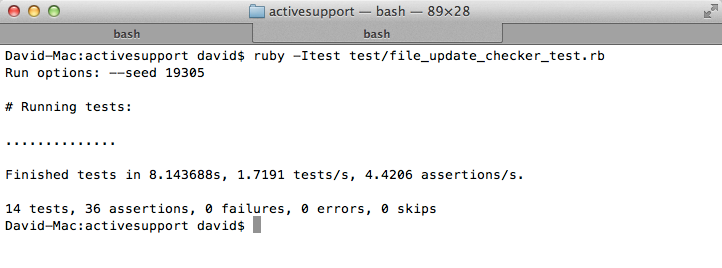
\includegraphics[width=0.8\textwidth]{images/test/fuc.png}
\caption{FileUpdateChecker测试结果}
\end{figure}
可以看到,FileUpdateChecker一共涉及14个测试用例共36个断言,且每个测试用例均已通过测试。

\subsection{MessageServer单元测试}
MessageServer单元测试的结果如下所示:

\begin{figure}[h]
\centering
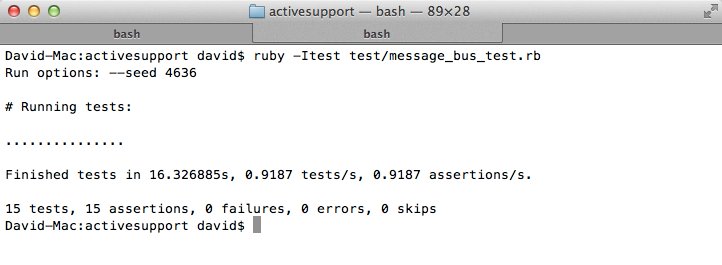
\includegraphics[width=0.8\textwidth]{images/test/msg.png}
\caption{MessageServer测试结果}
\end{figure}
可以看到,MessageServer一共涉及15个测试用例共15个断言,且每个测试用例均已通过测试。

\subsection{ActionController::Live单元测试}
ActionController::Live单元测试的结果如下所示:

\begin{figure}[h]
\centering
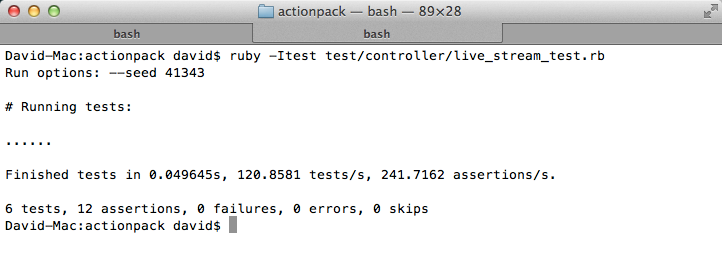
\includegraphics[width=0.8\textwidth]{images/test/live.png}
\caption{ActionController::Live测试结果}
\end{figure}
可以看到,ActionController::Live一共涉及6个测试用例共12个断言,且每个测试用例均已通过测试。

\subsection{ActionController::ServerSentEvents单元测试}
ActionController::ServerSentEvents单元测试的记过如下所示:

\begin{figure}[h]
\centering
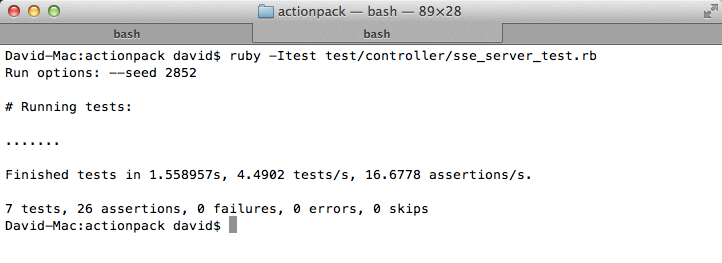
\includegraphics[width=0.8\textwidth]{images/test/sse.png}
\caption{ActionController::ServerSentEvents测试结果}
\end{figure}
可以看到,ActionController::ServerSentEvents一共涉及7个测试用例共26个断言,且每个测试用例均已通过测试。

\section{系统测试}
为了测试Rails消息总线技术的确能够正确工作,特别是测试Auto Reload以及Backend Instrumentation的功能正确性,本文采取了系统集成黑盒测试的方式。本文开发了一个测试用网站,该网站使用了Rails消息总线技术以及利用该技术实现的Auto Reload以及Backend Instrumentation技术特性,通过对该网站的功能性验证,能够验证Rails消息总线技术在系统级别上能够正常工作。

为了测试该技术,本文首先需要运行后台服务器。首先在命令行下将当前路径切换至测试网站的Rails工程目录下,再通过rails指令运行Rails服务器。如图\ref{fig-step1}所示:

\begin{figure}[h]
\centering
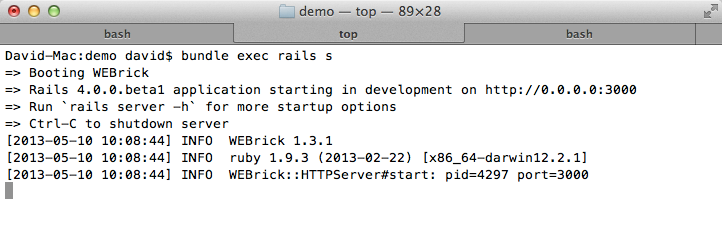
\includegraphics[width=0.8\textwidth]{images/test/1.png}
\caption{运行Rails技术测试网站}
\label{fig-step1}
\end{figure}

值得指出的是,这里使用bundle来间接的执行rails,其原因在于本文是通过对Rails的改进来实现大部分功能需求的,因此架设测试网站时不能使用当前Rails的正式发行版,只能指定执行本文的修改版Rails。使用bundle则是通过Gemfile配置文件告知整个系统使用本文提供的Rails版本。

另外,由于测试网站使用了Auto Reload技术和Backend Instrumentation技术,而该两种技术使用Gem形式打包封装的,需要首先在本技术测试网站的功能目录下找到Gemfile,并将该两个技术的Gem包含到这个工程中。这之后并且执行bundle install指令将其激活。

当命令行显示如图\ref{fig-step1}的内容时,则表示Rails服务器已经运行成功,技术演示网站已经正常上线,可以通过浏览器访问了。这时候切换操作系统至前台,打开浏览器,通过http://localhost:3000便可以访问测试网站,网站如图\ref{fig-step2}所示:

\begin{figure}[h]
\centering
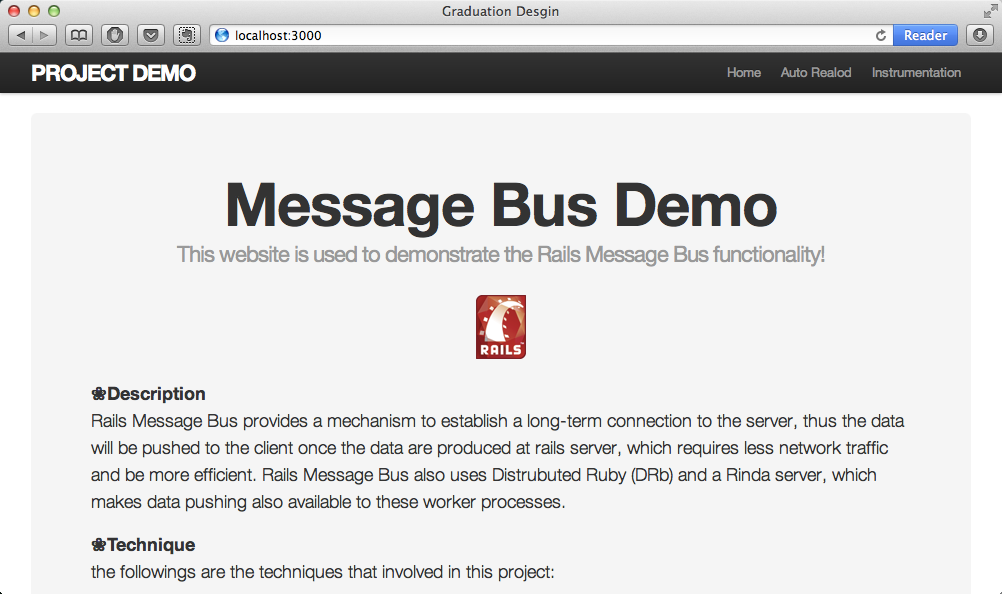
\includegraphics[width=0.8\textwidth]{images/test/2.png}
\caption{测试网站主页}
\label{fig-step2}
\end{figure}

下面需要测试Auto Reload的功能,首先通过浏览器地址栏键入地址http://localhost:3000/static\_demos/autoreload来访问该页面。页面载入后,其主要内容如图\ref{fig-step3}所示:

\begin{figure}[h]
\centering
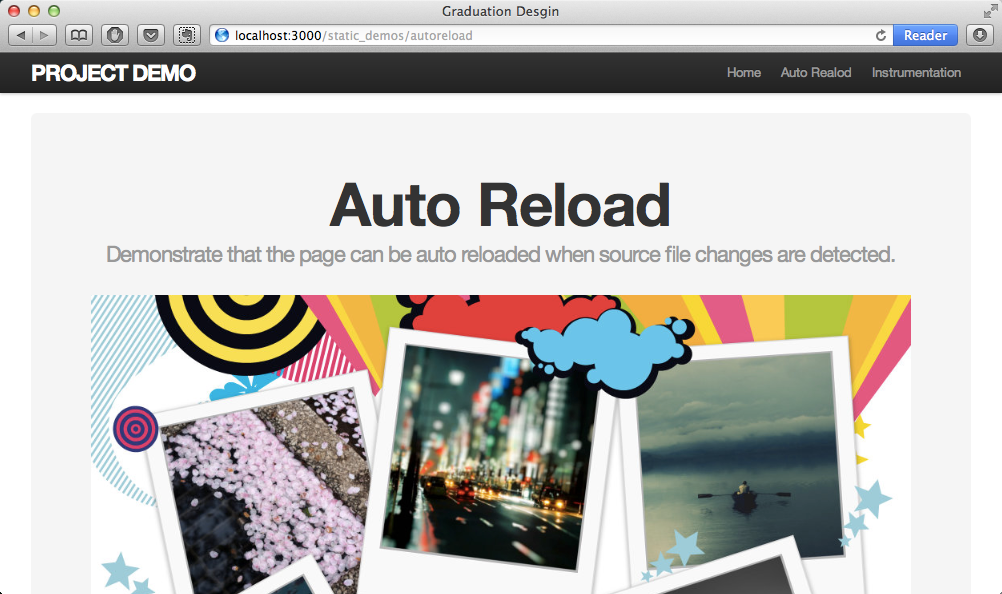
\includegraphics[width=0.8\textwidth]{images/test/3.png}
\caption{Auto Reload技术测试界面}
\label{fig-step3}
\end{figure}

可以看到,这个页面是一个非常简单的HTML页面,下面在后台找到该页面对应的HTML文件,并对其进行修改:

\begin{figure}[h]
\centering
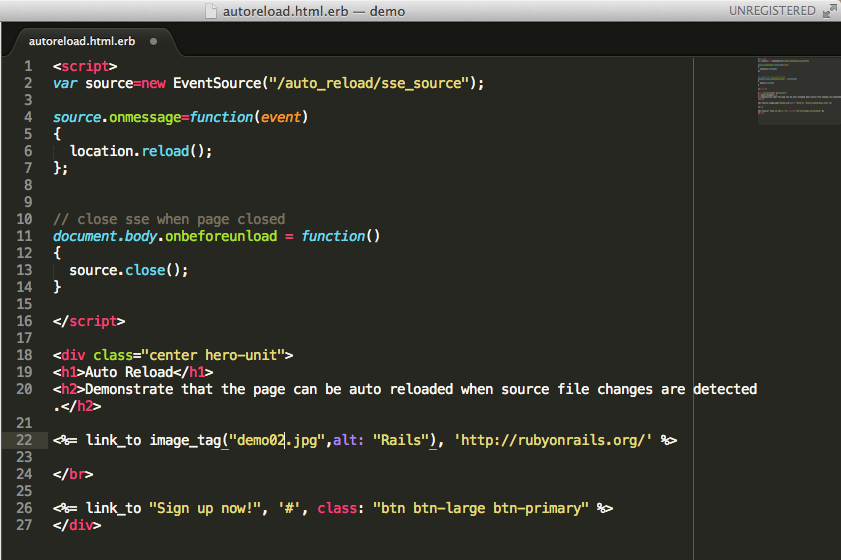
\includegraphics[width=0.8\textwidth]{images/test/4.png}
\caption{修改后台代码}
\label{fig-step4}
\end{figure}

后台的HTML文件实际上是是嵌入有Ruby代码的HTML文件,实际上,这是一个ERB(Embedded Ruby)文件该文件作为HTML文件的模板被执行,从而生成真正的HTML文件,并交给浏览器渲染。

作为测试示例,这里将图片标签进行更改。image\_tag是一个Ruby函数,它的调用将使得ERB生成HTML的IMG标签,用于显示一张图片。这里将展示的图片由原来的demo01.jpg更改到demo02.jpg,并保存。

这时候,Rails服务器中FileUpdateChecker检测到文件系统的该项变化,立刻通知消息总线将该消息传递给了前台页面。由于Auto Reload页面曾在后台订阅过该SSE消息,所以此时Auto Reload页面能够得知这一消息,从而进行自动刷新。可以看到,图\ref{fig-step5}是该页面自动刷新后的结果:

\begin{figure}[h]
\centering
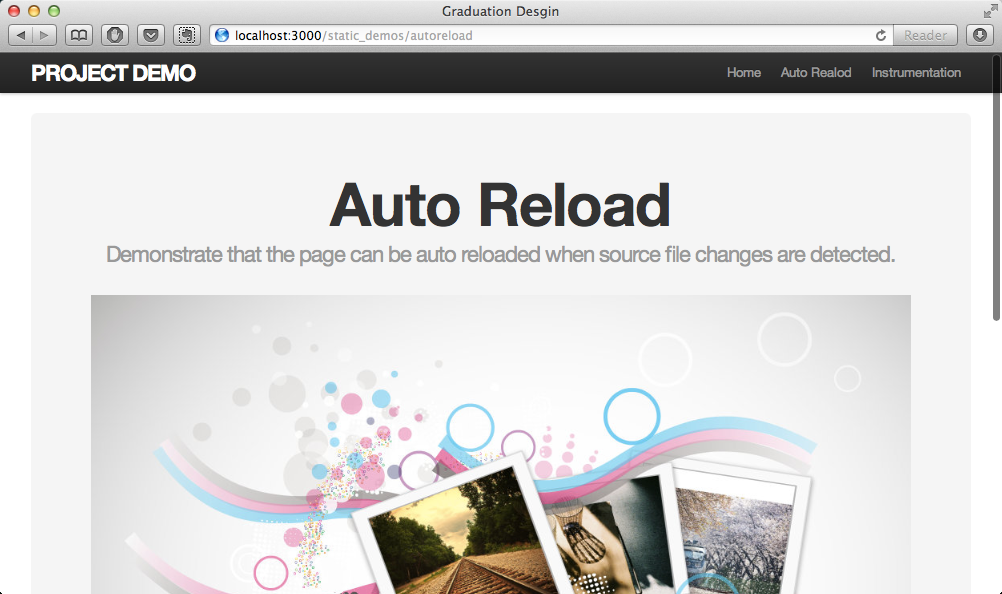
\includegraphics[width=0.8\textwidth]{images/test/5.png}
\caption{Auto Reload技术测试界面更新}
\label{fig-step5}
\end{figure}

以上便是Auto Reload的系统级别黑盒测试,下面将进行Backend Instrumentation的测试。通过访问http://localhost:3000/static\_demos/instrumentation进入该测试页面:

\begin{figure}[h]
\centering
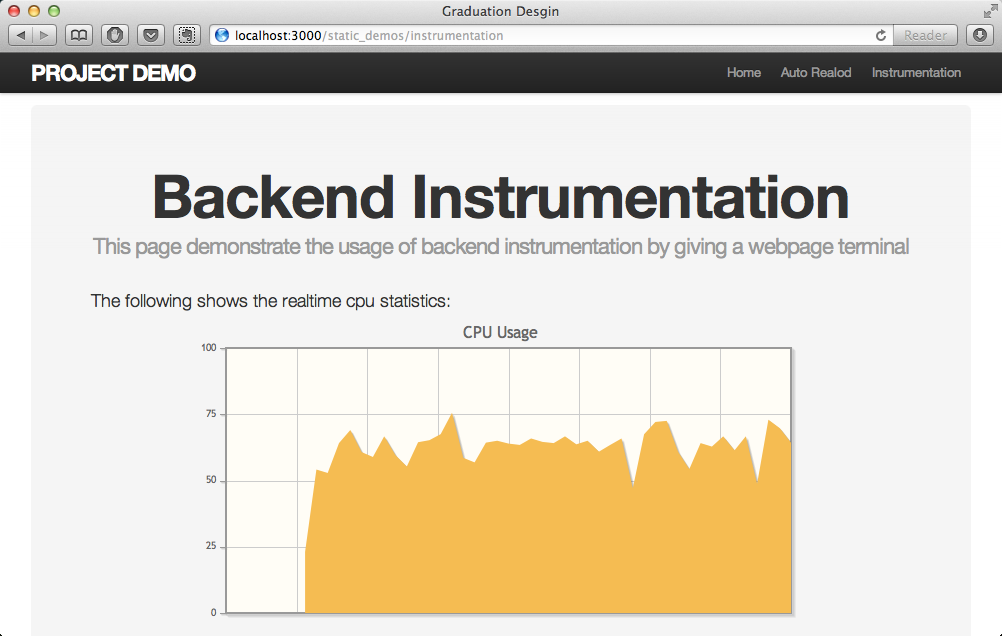
\includegraphics[width=0.8\textwidth]{images/test/6.png}
\caption{Backend Instrumentation技术获取后台CPU占用率}
\label{fig-step6}
\end{figure}

可以看到,在图\ref{fig-step6}中,首先展示了一个实时的图表,该图表用于实时的获取后台性能参数,并将其中后台CPU占用率的参数显示出来。除了后台CPU占用率,该页面还展示了实时的后台内存占用率情况:

\begin{figure}[h]
\centering
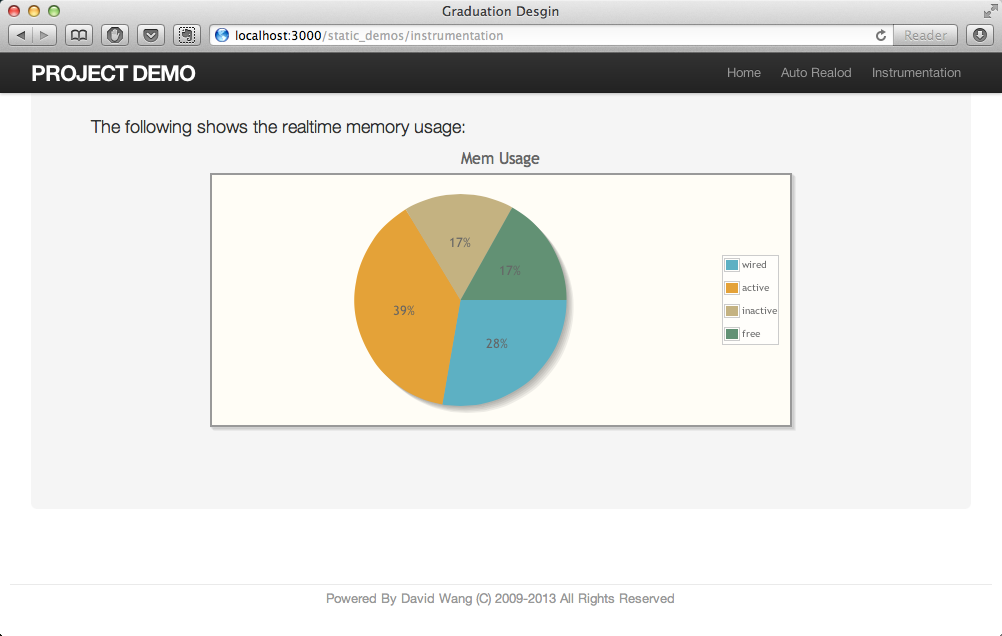
\includegraphics[width=0.8\textwidth]{images/test/7.png}
\caption{Backend Instrumentation技术获取后台内存占用率}
\label{fig-step7}
\end{figure}

以上,便是对Rails消息总线技术的功能性测试。结果表明,Rails消息总线技术能够正确实现其声称的功能。


